\documentclass[a4paper,12pt]{ report}
\usepackage[ top=2.5cm, bottom=2.6cm, left=3 cm, right=2.5cm]{geometry}
\usepackage{polski}
\usepackage[utf8x]{inputenc}
\usepackage{verbatim}
\usepackage{mathtools}
\usepackage{amssymb}
\usepackage{amsfonts}
\usepackage{amsthm} 
\usepackage{indentfirst}
\usepackage{graphicx}
\usepackage{tabularx}
\usepackage{longtable}

\usepackage{url}
\usepackage{enumerate}
\usepackage{color}
\usepackage{graphicx}
\usepackage{listings}
\usepackage{float}
\usepackage{array} % tabulator





%adres do obrazow
\graphicspath{{./obrazy/}} 


\definecolor{bgcolor}{rgb}{1.0,1.0,1.0} 		% kolor tla pod kodem
\definecolor{numbercolor}{rgb}{0.35,0.35,0.35} 	% kolor nr linii kodu
\definecolor{codecolor}{rgb}{0.20,0.20,0.20} 	% kolor kodu
\definecolor{keywordcolor}{rgb}{0.00,0.00,0.55}	% kolor slowa kluczowego
\definecolor{commentcolor}{rgb}{0.50,0.50,0.50}	% kolor komentarza w kodzie

% wyglad kodu w dokumencie
\lstset{
  basicstyle=\scriptsize
, keywordstyle=\color{keywordcolor}\bfseries
, commentstyle=\color{commentcolor}\slshape
, showstringspaces=false
, morekeywords={create, CREATE, fact, FACT ,dimension,DIMENSION,key,KEY pgloader,make, save_dir, user_namem, user_name, base_name, site_web,  exit},
, tabsize=1
, numbers=left
, numbersep=1.5em
, stepnumber=1
, xleftmargin=1.2em
, xrightmargin=1.2em
, breaklines=true
, breakatwhitespace=true
, frameround=fttt
, frame=BLtr
, framextopmargin=1ex
, framexbottommargin=1ex
, framexleftmargin=1ex
, framexrightmargin=1ex
, backgroundcolor=\color{bgcolor}
, breakautoindent=false
, belowcaptionskip=1.5ex
, inputencoding=utf8x
, extendedchars=\true
,   literate={ą}{{\k{a}}}1
             {Ą}{{\k{A}}}1
             {ę}{{\k{e}}}1
             {Ę}{{\k{E}}}1
             {ó}{{\'o}}1
             {Ó}{{\'O}}1
             {ś}{{\'s}}1
             {Ś}{{\'S}}1
             {ł}{{\l{}}}1
             {Ł}{{\L{}}}1
             {ż}{{\.z}}1
             {Ż}{{\.Z}}1
             {ź}{{\'z}}1
             {Ź}{{\'Z}}1
             {ć}{{\'c}}1
             {Ć}{{\'C}}1
             {ń}{{\'n}}1
             {Ń}{{\'N}}1
}

\widowpenalty=10000 %nie pozostawia wdów na ko«cu strony
\clubpenalty=10000 %nie pozostawia sierot
\brokenpenalty=10000 %nie dzieli stron jeżeli podział wyrazu


\def\noindentation{\let\@afterindentfalse}
\pagestyle{plain}


\linespread{1.5}
\setlength{\parindent}{1cm}
\newtheorem{mydef}{Definition}


% pomonce polecenia
\newcommand{\jezyk}		 {J($\mathbb{S} $)}
\newcommand{\slownik}[1] {$\mathbb{S}_{#1}$}
\newcommand{\zbior}	 	 {Z($\mathbb{S}$)}
\newcommand{\gramatyka}[1] {$\mathbb{G}_{#1}$}

\newcommand*\stdchapter{}
\let\stdchapter\chapter
\renewcommand*\chapter{%
\clearpage\ifodd\value{page}\else\mbox{}\clearpage\fi
\stdchapter}

\newcommand{\ang}[1]{ \textit{(ang. #1})}
\newcommand{\kategoria}[1]{$<$#1$>$}
\newcommand{\cytat}[1] { ''#1''}
\newcommand{\symlex}[1]{ \mbox{\uppercase{\textbf{#1}}}}
\newcommand{\defp}[1]{\textit{#1}}
%\newenvironment{akapit} %{} %{}

\begin{document}


\begin{center}

\begin{center}

\begin{figure}[h!]
  \begin{center}
    
\includegraphics[width=0.2\textwidth]{./logo_MiI.png}
  \end{center}
\end{figure}

\end{center}
\textsc{ \large Uniwersytet Łódzki\\
Wydział Matematyki i Informatyki \\
Instytut informatyki
}
\vskip 3cm
\end{center}
\begin{center}
{\Large \bf Andrzej Krupa }\\
 nr indeksu: 338689
\end{center}
\vskip 1cm
\begin{center}
{\Large \bf Język wysokiego poziomu do tworzenia procesów ETL w Hurtowniach danych.} \\
{ \large High-level language to create ETL process in data warehouse. }

\vskip 3cm
\begin{flushright}
Praca magisterska\\
przygotowana w Zakładzie Katedry Informatyki Stosowanej \\
promotor: dr Jan Pustelnik
\vskip 3cm

\end{flushright}
%\end{center}
%\vskip 4cm \hspace*{7cm}
%\parbox{10cm}{\Large
%Praca licencjacka\\
%napisana pod kierunkiem\\
%dr Jacek Krzaczkowski }
%\vskip 4cm
%\begin{center}
{\large \bf Łódź 2014}
\end{center}
\thispagestyle{empty}
\newpage\thispagestyle{empty}
\mbox{}
\newpage


\tableofcontents
\setlength{\parskip}{2ex plus 0.5ex minus 0.5ex}


\chapter*{Wstęp}
\addcontentsline{toc}{chapter}{Wstęp}

Ojcem koncepcji hurtowni danych jest Bill Inmon,
 napisał on ponad 40 książek związanych z tą tematyką.
Koncepcja ta dotyczy,
 jak wspomóc osoby zarządzające firmą,
 korporacją w podejmowaniu działań strategicznych.
Hurtownie danych odniosły sukces związany z problemami biznesowymi związanymi z zarządzaniem relacjami z~klientem,
 w~skrócie CRM, \ang{Customer Relationship Management}
Projektowanie jaki i tworzenie hurtowni danych jest procesem bardzo złożonym i~kosztownych,
 który trwa od pół roku do dwóch lat.
Firmy podejmujące decyzje o inwestycji utworzenia hurtowni danych,
 są świadome, 
 że nie produkt zakupiony ma generować zyski tylko dostarczać wiarygodnych i rzetelnych informacji, 
 na~podstawie których możliwe jest podjęcie decyzji strategicznych. 
Jeżeli projekt hurtowni danych jest nie ukierunkowany pod danego klienta lub przechowuje niepoprawne dane, 
 to staje się dużą stratą dla firmy.\cite{TodMan}

Celem pracy jest napisanie języka wysokiego poziomu, 
 który pomoże programistom w tworzeniu procesów zasilających hurtownie danych.
 Zadaniem owego języka, na podstawie podanych poleceń jest wygenerowanie:

\begin{itemize}
 \item szablonu pobierającego dane (źródło),
 \item szablonu pgloader lub gotowego polecenia insert,
 \item kodu umożliwiającego utworzenie tabeli,
 \item kodu języka SQL zasilającego tabele.
\end{itemize}

Pierwszy rozdział pracy opisuje hurtownie danych i powody jej budowania,
 jak również została przedstawiona w nim architektura hurtowni danych.
Kolejny rozdział opisuje, czym są procesy zasilania hurtowni danych, 
 oraz omawia przykładowe procesy zasilania, które są realizowane w ramach niniejszej pracy.
Trzeci rozdział niniejszej pracy został natomiast poświęcony teorii związanej 
z~tworzeniem języków interpretowanych.

Ostatni rozdział pracy dotyczy opisu programu wraz z przykładem.
 Wszystkie przykłady zamieszczone w niniejszej były testowane 
w składni języka SQL akceptowanego 
przez PostgreSQL 8.4.14 na systemie ubuntu 10.04 LTS.
Powodami wybrania bazy danych PstgresSQL jest:
\begin{itemize}
 \item bezpłatne oprogramowanie i uznane za dobre do zastosowań komercyjnych,
 \item wykorzystywane obecnie w firmie,
    w której zdobywam doświadczenie zawodowe pracując przy tworzeniu warstwy pośredniej hurtowni bazy danych.
\end{itemize}

Analizator składniowy i leksykalny został utworzony przy użyciu otwartego oprogramowania LEX i YACC, 
 które w znaczący sposób ułatwiają tworzenie pierwszych dwóch etapów tworzenia języków interpretowanych i kompilatorów.
Lex i Yacc są programami,
 które wymagają dużego nakładu pracy,
 by móc dobrze zrozumieć ich działanie i zalety jakich nam dostarczają w tworzeniu języka wysokiego poziomu.
Ponieważ celem niniejszej pracy nie jest tworzenie języków wysokiego poziomu,
 lecz napisanie go i aby nie odbiegać od głównego celu pracy
 opis działania jak również składni zostanie pominięty.

  


\chapter{Hurtownie danych}


Definicję Hurtowni Danych \ang{Data Warehouse}  przypisuje się Bill'owi Inmon'owi w 1992 roku.
Zgodnie z tą definicją Hurtownią danych jest bazą danych mającą następujące cztery cechy. \cite{TodMan}

\begin{itemize}
 \item Zorientowaną na temat \ang{ Subject-oriented} --- 
    dane są gromadzone 
    w~ściśle określonej dziedzinie, aby możliwe było zrobienie sensownego zestawienia danych.
   Nie są przechowywane działania czy operacje biznesowe. Hurtownia danych ograniczona w firmie do jednego działu 
    lub wybranego obszaru (np. Biznesowego),
    jest określana jako lokalna hurtownia danych 
    lub tematyczna hurtownia danych \ang{data mart} stanowiąca podzbiór hurtowni danych
 \item Nie ulotność \ang{Non-volatile} --- 
    dane przechowywane w Hurtowni danych nie są nigdy usuwane i modyfikowane, 
    przeznaczone są wyłącznie do odczytu w celu utworzenia raportu na podstawie zadanego zapytania SQL.
 \item integracja \ang{Intergrated} --- W hurtowni danych znajdują się informacje, 
   które pochodzą z całej firmy, przechowywanych w dowolnych technologiach,
   związku z~tym faktem musi wystąpić ujednolicenie typów danych.

 \item Zmienność w czasie \ang{Time-Variant} --- Na podstawie historii są podejmowane decyzje, musi zostać określone,
  co jaki okres czasu chcemy zapamiętać stan obecny w danej firmie.

\end{itemize}


\section{Powody budowania hurtowni danych.}
  
      Uzasadnieniem budowania hurtowni danych może być:
\begin{itemize}
 \item \textbf{Przeprowadzanie analizy danych bez ingerencji w operacyjną pracę systemów transakcyjnych.} --
    Analiza danych ze względu na bardzo dużą liczbę danych wymagają złożonych i czasochłonnych obliczeń.
    Dopuszczalne są zapytania kilku sekundowe, minutowe. Mogą wystąpić zapytania nawet kilku dniowe. 
    Zapytania te nie mogą wpłynąć na pracę systemu operacyjnego,
     w którym zapytanie nie może trwać dużej niż kilka sekund.
    (np. Użytkownik płacący kartą nie wie, czy odpowiedź o akceptacji przyjdzie za jedną sekundę, 
    czy za 2 minuty, czy za 5 minut.
    Jest to sytuacja nie dopuszczalna.)
\item \textbf{Całościowy wgląd w dane firmy} --
    Firmy posiadające dane na różnych środowiskach sprzętowych, w różnych aplikacjach zainstalowane.
    Posiada głębszą wiedzę na temat zdarzeń, które miały miejsce w jej firmie, jeżeli ma możliwość zintegrowania danych.
    Np. Pan K. ma sklep i warsztat samochodowy i~chciałby widzieć. 
    Ile sprzedanych części samochodowych i~kto naprawiał samochód w jego warsztacie, a kto nie.
\item \textbf{Dostęp do danych historycznych} -- 
   Dzięki danym historycznym możliwe jest wykonywanie analiz,
    z których można wyciągnąć wnioski, przekładające się na realne korzyści dla firmy.
\item \textbf{Ujednolicenie posiadanych informacji} -- 
   Eliminuje tzw. problem wielu wersji prawdy firmy. 
   Przedstawiony raport opiera się na podstawie jakiś danych. 
   Jeżeli dane pochodzą z różnych źródeł to są to wnioski osoby sporządzającej raport.
   Firma w jednym obszarze może prosperować bardzo dobrze,
    ale inny obszar może generować straty, które mogą być przyczyną upadku firmy.

\item \textbf{Przetwarzanie analityczne danych} \ang{On-Line Analytical Processing, OLAP} --  
  Z danych zgromadzonych w hurtowni danych są tworzone zestawienia statystyczne,
   wykresy i~raporty w~różnych okresach czasowych.
\item \textbf{Wspomaganie decyzji} \ang{Decision Support, DS} - wykonywanie 
  analizy symulującej scenariusz biznesowy. 
  
\end{itemize}


\subsection{OLAP a OLTP}
Przetwarzanie analityczne danych \ang{On-Line Analytical Processing, OLAP} 
 i~przetwarzanie transakcyjne \ang{On-Line Transactional Processing,  OLTP}
 są to systemy optymalizowane pod kątem przetwarzania danych. \cite{Vincent_Rainardi} \cite{TodMan}

System OLTP jest przeznaczony dla pracowników, komunikujących się 
 z Systemem bazodanowym w celu uzyskania informacji 
 np. sprawdzenie dostępnych miejsc na jakimś koncercie.

Podstawowymi cechami systemów OLTP są:
\begin{enumerate}
 \item wykonywanie przez wielu użytkowników bardzo dużej ilości zapytań, których czas realizacji jest krótki \label{OLTP_1},
 \item system bazodanowy powinien być zoptymalizowany pod kątem odczytu danych,
 \item częste usuwanie lub modyfikacja pojedynczych rekordów w bazie danych,
 \item dane przechowywane w bazie danych są zawsze aktualne.
\end{enumerate}

System OLAP jest przeznaczony dla pracowników przygotowujących zestawienie danych,
 raportów dla kadry zarządzającej, jak również dla analityków, 
 którzy na podstawie zadanych zapytań do hurtowni danych,
 mogą odkryć zależności występujące w firmie, a następnie wyciągnąć odpowiednie wnioski,
 które w ich opinii mogą dać firmie zysk.
 
Podstawowymi cechami systemów OLAP są:
\begin{enumerate}
 \item wykonywanie przez nie wielką liczbę użytkowników małej ilości zapytań na dużym obszarze danych,
 \item cyklicznie zasilane w ustalonych przedziałach czasowych,
 \item dane w bazie nie muszą być aktualne w czasie rzeczywistym.
\end{enumerate}


\subsection{Wspomaganie decyzji }
Systemy wspomagania decyzji \ang{decision support systems} tworzone są 
 w celu szukania minimalizacji kosztów prowadzonej działalności,
 lepszego przewidywania ryzyka podejmowanych działań, podniesienia jakości obsługi klienta. System OLAP jest 
 jednym z takich narzędzi, które wspierają podejmowanie decyzji.
Przykładowymi pytaniami na które system powinien odpowiedzieć są\cite{TodMan} :
 \begin{enumerate}
  \item Jaki był dochód w rozbiciu na poszczególnych klientów?
  \item Jaki był procentowy wzrost lub spadek dochodu w porównaniu z zeszył miesiącem?
  \item Jakie są cech najlepszych/najgorszych klientów (cechy klientów muszą być ściśle określone)?
  \item Listę klientów, dla których współczynnik odejścia jest wysoki, a przynoszą zysk firmie.
 
 \end{enumerate}

Hurtownie danych odniosły sukces związanym z zarządzanie relacjami z klientem 
 \ang{Customer Relationship Management, CRM}, które mają na celu zatrzymanie najlepszych klientów,
 sprzedawanie im większej liczby produktów, jak również pozyskiwanie nowych klientów.

\section{Architektura hurtowni danych} \label{p_temat}
  W niniejszym podrozdziale zostanie przestawiona podstawowa architektura hurtowni danych oraz 
   proces związany z tworzeniem hurtowni, który jest bardzo drogi, czasochłonny 
   i~żeby osiągnął sukces musi on być ukierunkowany na klienta, czyli pod jego wymagania, 
   które opierają się na intuicji.
   Na rysunku \ref{fig:AHD} przedstawia główne elementy hurtowni danych oraz kierunek przepływu danych. Przy użyciu 
   strzałek został pokazany przepływ danych.\cite{TodMan} \cite{link_hd}

\begin{center}
\begin{figure}[H]
  \begin{center}
    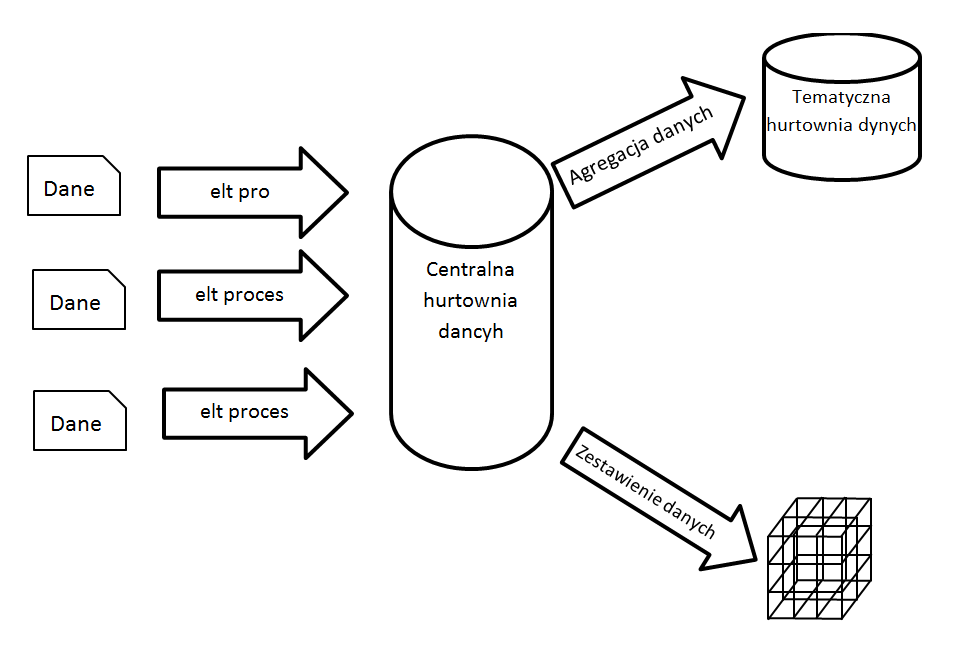
\includegraphics[width=0.7\textwidth]{AHD.png}
  \end{center}
 \caption{Architektura hurtowni danych. }
    \label{fig:AHD}
\end{figure}
\end{center}


Strukturę przepływu danych możemy podzielić na:
\begin{itemize}
 \item \textbf{Źródło danych \ang{source} } --- 
    są to dane, które będą pobierane do hurtowni danych 
 \item \textbf{proces ETL \ang{extract, transfer, load} } --- 
    procesem elt nazywamy czynności wykonywane w celu pobrania danych źródłowych
    przekształcenie w odpowiedni format danych, a następnie umieszczeni ich w centralnej hurtowni danych,
    proces elt dokładnie będzie omówiony w rozdziale drugim.
 \item \textbf{centralna hurtownia danych \ang{center data  warehouse}} --- 
    jest to miejsce docelowe przetworzonych danych ze źródeł,						                                          
 \item \textbf{hurtownie tematyczne \ang{data marts}} --- 
    zawierają wybrane dane z centralnej hurtowni danych w~sposób 
    zagregowany, umożliwiające szybkie operowanie sporządzanie raportów,
 \item \textbf{zestawienie danych } --- 
    docelowym produktem hurtowni danych jest tworzenie odpowiednich zestawień danych.
    Na rysunku \ref{fig:AHD}, został przedstawiona jako kostka.
\end{itemize}

 
Tworzenie hurtowni danych jest stosunkowo młodą dziedziną, która się dynamicznie rozwija.
Dzięki zastosowaniom CRM odniosły one sukces co spowodowało większe zapotrzebowanie na przechowywanie
 i~analizowanie danych historycznych. Przedstawiona architektura danych na rysunku \ref{fig:AHD}, 
 nie spełnia swojej roli dla Hurtowni Danych, w których przyrost  danych jest bardzo duży.\cite{link_hd}
Poniżej została przedstawione inna architektura danych.
\begin{center}
\begin{figure}[H]
  \begin{center}
    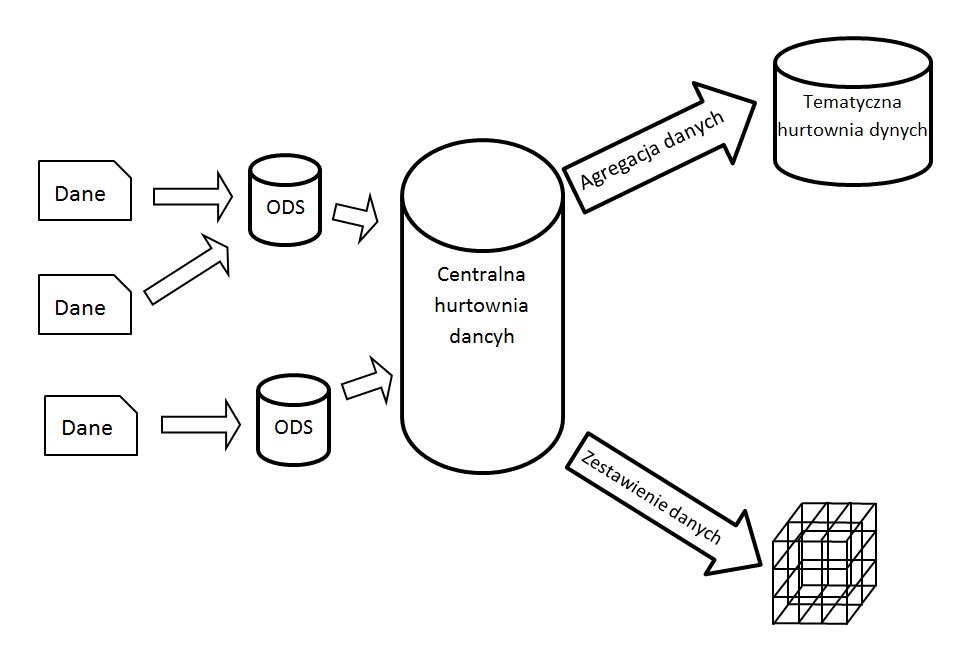
\includegraphics[width=0.7\textwidth]{AHD_ODS.png}
  \end{center}
  \caption{Architektura hurtowni danych z magazynem danych ODS. }
    \label{fig:ODS}
\end{figure}
\end{center}

Do architektury z rysunku \ref{fig:AHD} został dodany magazyn danych operacyjnych \ang{operational data store, ODS}, który
pełni role magazynu danych. Ładowane są do niej dane pobrane ze źródeł i przetworzone w celu uzyskania zgodności typów danych.
Kolejnym etapem jest załadowanie danych w sposób zagregowany do centralnej hurtowni danych.


\section{Projektowanie hurtowni danych.}
Projektowanie hurtowni danych tak jak relacyjnych baz danych polega na utworzeniu następujących modeli\cite{TodMan}:

\begin{itemize}
 \item \textbf{Model pojęciowy} --- 
    przy użyciu języka biznesowego w danej firmie opisuje się cele biznesowe, 
    które będzie można określić przez gromadzenie ściśle określonych danych.
   Na modelu pojęciowym powinny, być zaznaczone nazwy kolumn, które mają być przechowywane 
    w tabeli znajdującej się w Hurtowni Danych
 \item \textbf{Model logiczny} --- 
    jest to opis elementów  logicznych hurtowni danych, wykonany np. w języku UML.
 \item \textbf{Model fizyczny} --- 
    jest to opis indeksowania, partycjonowania, opis sprzętu komputerowego, sieci
     rozmieszczenie poszczególnych zasobów fizycznych.
\end{itemize}

Najpopularniejszymi metodami przyjętymi podczas tworzenia hurtowni danych są:
\begin{itemize}
 \item \textbf{Projektowanie wstępujące} (od szczegółu do ogółu)---
    Polega na tworzeniu wszystkich etapów hurtowni danych
    jednocześnie, a następnie na integracji poszczególnych etapów ze sobą.
 \item \textbf{Projektowanie zstępujące} ---
    Dopóki jeden etap tworzenia hurtowni danych się nie skończy, 
     to następny się nie zacznie.
    Jeżeli pojawią się błędy to wraca się do poprzedniego etapu i zaczyna się prace 
     na kolejnym etapie od nowa.
\end{itemize}



\section{Wielowymiarowy danych danych}
Wielowymiarowym modelem danych \ang{Multidimensional Data Model} 
nazywamy dane zorganizowane w:
\begin{itemize}
 \item \textbf{fakt \ang{facts}  } --- 
    są to dane opisujące jakieś zdarzenie, 
    tabelkę przechowującą te dane nazywamy  \textit{tablicą faktów} 
   Fakt opisany jest przez wymiary i miary,
 \item \textbf{wymiar \ang{dimension}} --- 
    Jest jakąś cechą opisującą dany fakt, cechy te znajdują się w tablicy wymiarów i są opisane przez atrybuty,
 \item \textbf{atrybut} \ang{ attribute}  --- 
    Przechowuje dodatkowe informację na temat wymiaru,
 \item \textbf{miara \ang{measures}} --- 
    Jest wartością mierzalną przypisaną do pojedynczego rekordu w tablicy faktów. 
\end{itemize}

Model ten jest zintegrowaną częścią z systemem OLAP.
Podstawowym atutem wielowymiarowego modelu danych jest proste zrozumienie hurtowni danych 
 i poruszania się po niej w sposób efektywny, szybsze wykonywanie zapytań zadawanych do hurtowni danych, 
Jak również możliwość analizy danych w różnych wymiarach, 
które jest bardzo istotne ze względów biznesowych:
\begin{itemize}
 \item Oglądanie informacji rozłożonych w czasie,
 \item Wyświetlanie informacji w sposób graficzny,
 \item Możliwość zmiany przekroju danych w dowolny sposób,
 \item Analizę danych pod kątem informacji istotnych dla danej firmy.
\end{itemize}

Podstawowymi schematami wielowymiarowego modelu danych są:
\begin{itemize}
 \item schemat gwiazdy \ang{Star schema} 
 \item schemat płatka śniegu \ang{Snowflake schema}
\end{itemize}

\subsection{Schemat gwiazdy}
Schemat gwiazdy jest podstawowym schematem wielowymiarowego modelu danych,
 w którym znajduje się jedna tabela faktów połączona z wieloma tabelami wymiarów.
Tabela faktów w tym schemacie jest w trzeciej postaci normalnej, a tabela wymiarów jest w drugiej postaci normalnej,
dzięki takiej strukturze możliwe jest szybsze przeglądanie danych poprzez \cite{TodMan} \cite{link_hd}:
\begin{itemize}
 \item poszczególne wymiary,
 \item sumowanie danych,
 \item agregację danych,
 \item filtrowanie danych
\end{itemize}

Na rysunku  \ref{fig:gwiazda} został przedstawiona przykładowa architektura schematu gwiazdy.
\begin{center}
\begin{figure}[H]
  \begin{center}
    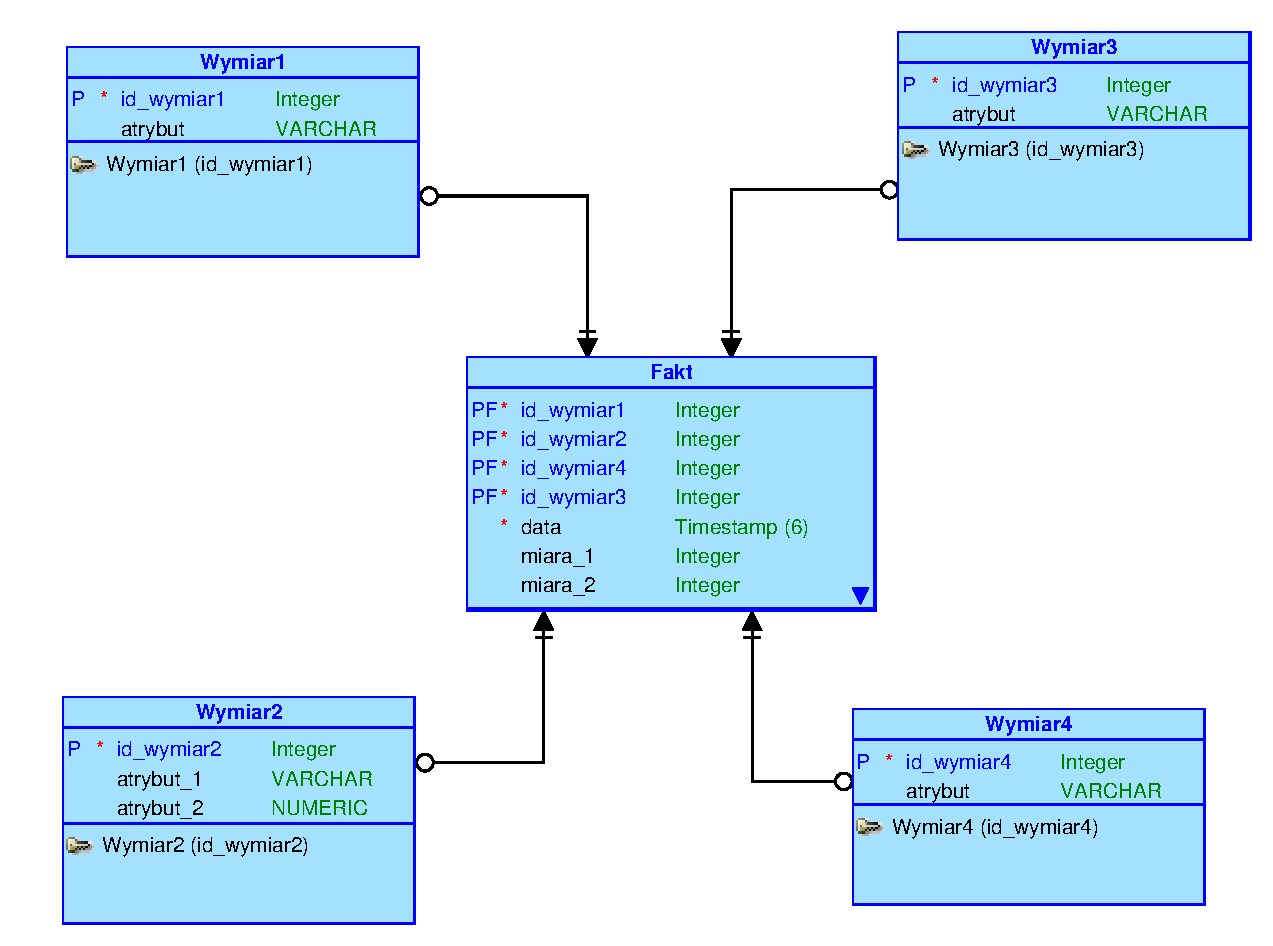
\includegraphics[width=0.7\textwidth]{gwiazda.pdf}
  \end{center}
  \caption{Przykładowy schemat gwiazdy w postaci abstrakcyjnej. }
    \label{fig:gwiazda}
\end{figure}
\end{center}
Poniżej znajduje się listing zapytań do bazy danych w języku postgresql,
 który realizuje model logiczny gwiazdy zawarty na rysunku \ref{fig:gwiazda}
\lstinputlisting[language=sql, caption = {Listing kodu tworzący schemat gwiazdy. } ]{"./sql/gwiazda.sql"}

\subsection{Schemat płatka śniegu}
Architektura schematu gwiazdy jest uproszczoną formą architektury płatka śniegu.
Podstawową różnicą pomiędzy tymi schematami jest tabela wymiarów, która jest znormalizowana.

Schemat płatka śniegu jest stosowany wtedy, gdy tabela wymiarów osiąga duży rozmiar.
Normalizuję się tabele wymiarów, aby zmniejszyć jej liczebność, dzięki czemu czas zapytań, 
powinien się znacząco skrócić. 
Wadą tego podejścia jest, że im bardziej znormalizowana jest tabela wymiarów,  
to tym bardziej skomplikowane łączenia SQL muszę zostać użyte, aby pobrać odpowiednie
dane z hurtowni danych. \cite{TodMan} \cite{cube}

Przykładowa architektura płatka śniegu został przedstawiona na rysunku \ref{fig:platek_sniegu} .

\begin{center}
\begin{figure}[H]
  \begin{center}
    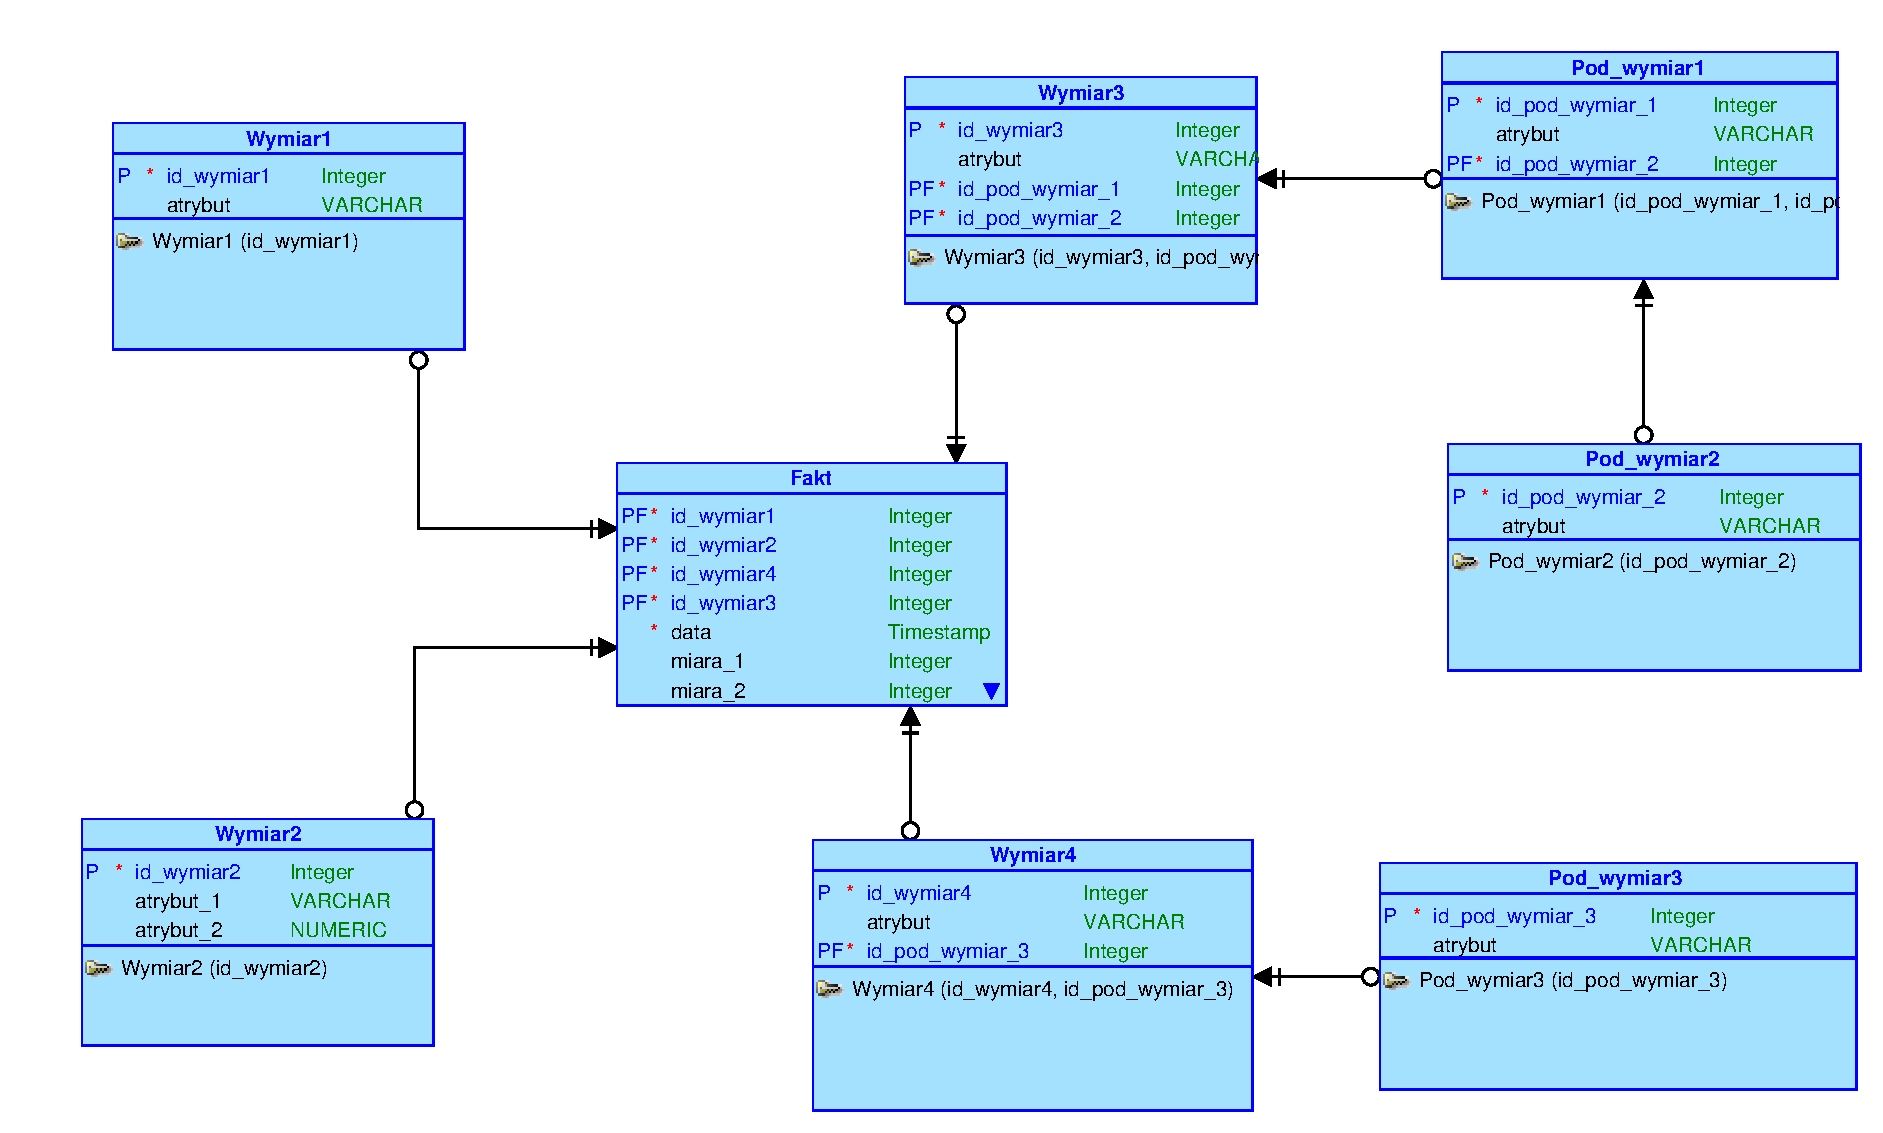
\includegraphics[width=0.7\textwidth]{platek_sniegu.pdf}
  \end{center}
  \caption{Przykładowy schemat płatka śniegu w postaci abstrakcyjnej. }
    \label{fig:platek_sniegu}
\end{figure}
\end{center}







\begin{comment}
 
\end{comment}

\chapter{Procesy zasilania hurtowni danych} \label{r_procesy}

\section{Ogólna koncepcja zasilania hurtowni}
Hurtownia danych jako system magazynujący dane i wspierający raportowanie stawia sobie 
 jako jeden z głównych celów gromadzenie danych i takie ich przekształcanie,
 aby przyszłe raportowanie było jak najłatwiejsze w kontekście pytań biznesowych,
 jakie stawiają użytkownicy końcowi.
Ogół procesów zasilania jest najczęściej określany skrótem ETL,
 pochodzącym od angielskich słów Extract, Transform, Load (ekstrakcja, transformacja, ładowanie),
 które oddają charakter procesów,
 oraz podsumowują cele,
 jakie są stawiane przed procesami zasilania hurtowni danych.


\subsection{Ekstrakcja}
Dane, które ostatecznie trafiają do hurtowni,
 pochodzą z różnych źródeł w firmie lub poza nią i różnią się sposobem dostępu.
Źródłami mogą być systemy transakcyjne (transakcje bankowe, system płatności online, systemy obsługi klienta,
 zapisy partii szachowych online itp.),
 logi systemów (logi stron internetowych,
 systemów e-commerce,
 pliki z wykazem połączeń telefonicznych),
 publicznie dostępne pliki 
 (dane giełdowe, wskaźniki i dane makroekonomiczne GUS czy nawet ręcznie generowane przez użytkowników biznesowych 
 (arkusze kalkulacyjne, plany i cele sprzedaży).
Różnorodność źródeł stawia po stronie hurtowni danych konieczność ekstrakcji danych z formatu,
 w którym są dostępne,
 niezależnie od źródła i formatu 
 (pliki tekstowe, bazy danych, arkusze kalkulacyjne, dane nieustrukturyzowane, obrazy itp.).
Czasami trudność przedstawia samo znalezienie właściwego źródła danych,
 bądź znalezienie kilku źródeł, które razem zawierają potrzebne informacje,
 czasami najtrudniejsze jest wykonanie ekstrakcji 
 (zwłaszcza, jeśli mamy do czynienia z wiekowymi systemami pisanymi kilkadziesiąt lat temu w języku COBOL na komputerach klasy mainframe 
 --- wbrew pozorom tego typu systemy są jeszcze w użyciu).
Mogą również pojawić się problemy wydajnościowe związane z transportem danych 
 (
   np. danych jest na tyle dużo,
   że wąskim gardłem staje się przepustowość sieci 
   i należy uciec się do kompresji danych jako do rozwiązania problemu
 ).
Jednym z problemów do rozwiązania przy ekstrakcji danych jest minimalizacja wpływu procesów ekstrakcji na funkcjonowanie źródła danych 
 --- zazwyczaj systemy transakcyjne nie potrafią sobie poradzić z pobieraniem dużej ilości danych, 
 gdyż same z siebie są zoptymalizowane do szybkich przetwarzań niewielkich ilości danych.
Może okazać się, że próby ekstrakcji danych bezpośrednio z systemu źródłowego są tak wielkim obciążeniem wydajnościowym,
 że doprowadzają do nieakceptowalnych czasów działania systemu transakcyjnego.
Do typowych rozwiązań należy harmonogramowanie procesów ETL w taki sposób,
 by ekstrakcja odbywała się np. w nocy,
 kiedy użytkowników systemu transakcyjnego jest mniej lub nie ma ich wcale, 
 oraz korzystanie z kopii systemu źródłowego dla celów ekstrakcji 
 (np. druga baza danych połączona z pierwszą w system „hot standby” 
 lub po prostu zwykła kopia odtwarzania z codziennych backupów systemu transakcyjnego.


\subsection{Transformacja}
Po pobraniu danych, dane muszą zostać przekształcone do wspólnej postaci.
Wynika to z faktu, że różne źródła, nawet podobne do siebie,
 przechowują dane w różnej postaci i zakładają różne zależności pomiędzy poszczególnymi elementami. 
Na przykład, bank powstały w wyniku fuzji kilku innych banków może korzystać z kilku systemów obsługi klienta. 
W jednym systemie kluczowi klienci biznesowi mogą mieć przypisanego jednego opiekuna
 i taka bieżąca informacja jest dostępna w systemie źródłowym,
 modelowana jako relacja jeden do wielu (jeden opiekun dla wielu klientów), 
 natomiast w drugim systemie może to być relacja wiele do wielu z archiwizacją historii przypisań opiekunów do klientów.
Dane w systemach transakcyjnych bardzo często są zgodne z trzecią postacią normalną,
 natomiast hurtownia danych często przechowuje i prezentuje dane w postaci zdenormalizowanej,
 zwłaszcza jeśli do modelowania hurtowni został wybrany schemat gwiazdy. 
Kontynuując przykład opiekuna klienta, model hurtowni danych może przewidywać opiekuna jako zwykły atrybut klienta,
 ignorując fakt, że w rzeczywistości relacja jest postaci jeden do wielu bądź wiele do wielu i tak jest zamodelowana w systemach źródłowych. 
Tego typu transformacje oraz zamiany kluczy z systemów źródłowych na własne klucze używane przez hurtownię 
(zazwyczaj zwane w środowisku hurtowni danych kluczami sztucznymi) są podstawowymi zadaniami procesów zasilania hurtowni.
Do innych typowych przekształceń należy tworzenie wspólnych typów danych 
 (np. ten sam atrybut może być opisywany w różnych systemach przez ciągi znaków różnej długości),
 ujednolicanie zawartości atrybutów 
 (np. typ klienta może przybierać wartości „biznesowy”, „business”, 3, „firma” itp. w różnych systemach,
 w hurtowni chcemy przechowywać jedną wartość, wspólną dla wszystkich rekordów jednego typu),
 łączenie bądź rozdzielanie atrybutów (np. „małżeństwo z dziećmi” chcemy rozdzielić na dwa atrybuty,
 jeden opisujący „małżeństwo”, drugi niosący informację, czy „ma dzieci”),
 łączenie atrybutów (np. rodzaj „firma”, rozmiar „poniżej 200 pracowników” chcemy oznaczyć jako „SME”).
 Możliwe są również przekształcenia specyficzne dla danej dziedziny,
 np. wyliczanie stopy zwrotu czy procentowej zmiany cen z danych giełdowych.


\subsection{Ładowanie}
Przekształcone dane muszą trafić do docelowego modelu danych.
Większość pracy została już wykonana na etapie ekstrakcji i transformacji,
 jednak pozostaje zadbać o spójność danych 
 (czy podczas ładowania hurtownia pozwoli na dostęp do transakcji dla nowych klientów,
 których jeszcze nie zdążyliśmy załadować?).
Często tego typu kwestie są rozwiązywane w zupełnie inny sposób niż w systemach transakcyjnych,
 w których spójność danych jest zapewniana mechanizmami bazodanowymi typu transakcje czy więzy integralności.
Przenoszenie takich rozwiązań do hurtowni danych stwarza potencjał dla problemów wydajnościowych zależnych bądź nie od implementacji
 konkretnego systemu zarządzania bazami danych – np. więzy integralności spowalniają ładowanie,
 gdyż są sprawdzane wiersz po wierszu,
 a transakcje czasami wręcz nie są możliwe do użycia 
 z uwagi na ograniczenia techniczne przy dużej ilości danych przetwarzanych w hurtowniach. 
Przykładowo, w systemie zarządzania bazą danych Oracle,
 transakcje standardowo generują UNDO i REDO,
 więc zawarcie całości ładowania w jednej transakcji,
 nawet gdyby było technicznie możliwe 
 (bazę można skonfigurować, aby udostępniała wystarczająco dużo miejsca na UNDO i REDO), 
 stwarzałoby olbrzymie problemy wydajnościowe z uwagi na kilkukrotne zwiększenie ilości operacji wejścia/wyjścia 
 (należy pamiętać, że UNDO też jest chronione przez REDO,
 więc ilość operacji dyskowych może wzrosnąć nawet czterokrotnie). 
Typową „sztuczką” praktyczną bywa np. wyłączenie generowania REDO na poziomie bazy danych. 
Jeśli chodzi o UNDO,
 to typowym rozwiązaniem jest podzielenie transakcji na mniejsze części,
 co redukuje ilość UNDO, które musi być przechowywane 
 (każde zatwierdzenie transakcji pozwala na pozbycie się UNDO,
 które zostało wygenerowane przez daną transakcję), 
 ale to już oznacza,
 że zapewnienie spójności musi leżeć po stronie procesów zasilania. 
Na szczęście zasilanie hurtowni danych jest procesem wsadowym, który w razie czego może zostać powtórzony,
 więc większość tradycyjnych mechanizmów bazodanowych zapewniających ochronę transakcji nie jest potrzebna. 
Zapewnienie spójności danych jest realizowane w samych procesach ładowania, 
 chociażby przy ustalaniu kolejności zasileń.
Przykładowo, ładując hurtownię zbudowaną w oparciu o schemat gwiazdy, 
 tradycyjnie ładuje się najpierw wymiary, 
 a potem fakty. Pomimo że nie zapewnia to spójności w najściślejszym znaczeniu tego pojęcia 
 (mogą pojawiać się wiersze w tabelach wymiarów, które nie mają swoich odpowiedników w tabelach faktowych), 
 to w praktyce jest to spójność, jakiej oczekują użytkownicy i personel utrzymujący hurtownie danych.
Wynika to z faktu, że w modelu gwiazdy wymiary są używane do interpretacji danych faktowych, a więc ich znaczenie jest drugorzędne. 
Najbardziej istotne jest, aby wszystkie dane faktowe dostępne dla użytkownika były opisane przez wymiary, 
więc ładowanie wymiarów w pierwszej kolejności zapewnia ten stan rzeczy. 


\section{Analiza przykładowego procesu zasilania} \label{p_r_analiza_procesu}
Dla zilustrowania koncepcji języka do budowy hurtowni danych oraz jego praktycznego zastosowania,
 zostanie zbudowana przykładowa,
 uproszczona hurtownia danych wraz z procesami zasilania. 
Tematyką hurtowni będą dane giełdowe,
 a konkretnie notowania ciągłe z warszawskiej Giełdy Papierów Wartościowych (GPW).
Wybór ten jest umotywowany powszechną dostępnością danych ---
 każdy może sobie w dowolnej chwili pobrać publicznie dostępne dane z wielu różnych stron internetowych.
Nie bez znaczenia jest również prostota danych, które są intuicyjnie zrozumiałe dla większości osób 
 i~nie będą wymagały wyjaśniania.

Do zbudowania hurtowni danych zostanie użyty schemat gwiazdy, 
 w którym występować będzie jedna tabela faktów, zaprezentowana na listingu \ref{l:fakt},
 wraz z towarzyszącym jej wymiarem pokazanym na listingu \ref{l:wymiar}.
\lstinputlisting[ label=l:fakt,  language=sql, caption ={Kod tworzący tabelę faktów. }]{"./sql/fakt_tabela.sql"} 
\lstinputlisting[ label=l:wymiar, language=sql,caption ={Kod tworzący tabelę wymiaru.}] {"./sql/wymiar_tabela.sql"} 

 
Docelowe rozwiązanie będzie składało się z trzech warstw:
 \begin{itemize}
  \item warstwy interfejsowej,
  \item warstwy pośredniej,
  \item warstwy docelowej,
 \end{itemize}
które zostaną omówione w kolejnych podrozdziałach.

\subsection{Warstwa interfejsowa}

Warstwa interfejsowa będzie służyła do komunikacji ze światem zewnętrznym celem pobrania danych do hurtowni. 
Przed procesami zasilania będą postawione następujące zadania szczegółowe:
\begin{enumerate}
 \item \label{w_intf:wykrywanie}
 Wykrywanie nowych danych w systemie źródłowym
 \item \label{w_inf:pobieranie}
 Pobieranie danych z systemu źródłowego
 \item \label{w_intf_ladowanie}
Ładowanie plików do bazy danych                 
        
\end{enumerate}

Dane o cenach akcji GPW są publicznie dostępne w internecie 
 i są już wyekstraktowane w postaci gotowych do ściągnięcia plików tekstowych.
Zatem nie jest konieczne, aby procesy zasilania wykonywały ekstrakcję ze źródła (jakiegoś systemu operacyjnego).
Zamiast tego, przydatne będzie wykrywanie,
 czy od ostatniego wykonania procesów zasilania pojawiły się nowe pliki z danymi 
 i pobranie wyłącznie nowych danych.
 
Cel ten zostanie zrealizowany za pomocą skryptów powłoki systemu Linux,
 (przedstawiony na listingu)
 oraz podstawowych narzędzi systemowych dostępnych z poziomu systemu operacyjnego. 


\lstinputlisting[ label=l:skrypt, language=sh, caption = {Skrypt pobierający dane serwera bossa.pl .}] {"./skrypt/skrypt_gpw.sh"} 


Procesy ETL muszą pobrać dane i przygotować do ładowania. 
Są to wszystkie czynności, które programiści uznają za potrzebne 
 w celu przygotowania danych do poprawnego załadowania danych do tabelki interfejsowej.
Czynnościami tymi może być chociażby rozpakowanie danych i rozmieszenie ich w odpowiednich katalogach.
W naszym rozważanym przykładzie pobieramy plik o nazwie \textit{sesjacgl.prn},
 który jest plikiem tekstowym.

Pliki muszą zostać załadowane do bazy danych w niezmienionej formie, celem ich udostępnienia do dalszych przekształceń.
Trafiają one do tabelki interfejsowej,
 która ma typ zmiennych zgodny z pobranymi danymi źródłowymi. 
Tabelkę te nazywać będziemy \textit{intf\_pgw},
 a ma ona strukturę zaprezentowaną na listingu \ref{l:t_intf_gpw} .

\lstinputlisting[ label=l:t_intf_gpw, language=sql, caption = {Kod tworzący tabelkę interfejsową.}] {"./sql/tworz_intf_gpw.sql"} 


Dla umożliwienia pełnej audytowalności procesów,
 konieczne jest przechowywanie ściągniętych plików przynajmniej przez jakiś czas.
W razie wystąpienia wątpliwości odnośnie jakości danych,
 będzie możliwość weryfikacji danych i porównania hurtowni z danymi źródłowymi. 
Często w hurtowniach danych istnieje dedykowana warstwa służąca tylko temu celowi. 
W rozwiązaniu zbudowanym na potrzeby niniejszej pracy,
 archiwizacja będzie odbywać się za pomocą kompresji plików i przeniesienia ich do dedykowanego katalogu, 
 co zostało pokazane na listingu \ref{l:skrypt}. 
 
W komercyjnych rozwiązaniach, jeśli archiwizacja danych odbywa się za pomocą plików,
 najczęściej stosowane są specjalistyczne narzędzia do backupów,
 a dane ostatecznie nagrywane są na taśmy.
Z uwagi na wysoką cenę tego typu urządzeń 
 oraz łatwą publiczną dostępność danych źródłowych użytych na potrzeby niniejszej pracy, 
 taki poziom dbałości o bezpieczeństwo danych nie jest konieczny. 

W celu załadowania danych do bazy danych zostanie użyte narzędzie pgloader,
 które dobrze współpracuje z systemem zarządzania bazą danych PostgresSql.
Na listingu \ref{l:pgloader} został pokazany skrypt pgloader'a , który realizuje to zadanie.

\lstinputlisting[ label=l:pgloader, language=sh, caption = {Skrypt pgloader'a ładujący dane do tabelki interfejsowej.}] {"./skrypt/pgloader.conf"}


\subsection{Warstwa pośrednia}

Celem warstwy pośredniej jest przekształcenie danych z formatu źródłowego, które znajdują się w tabeli interfejsowej,
czyli w tabeli \textit{intf\_gpw}, pokazanej na listingu \ref{l:t_intf_gpw},
na format umożliwiający załadowanie danych do tabeli docelowej.
Szczegółowe cele zależą najczęściej od konkretnego rozwiązania i jego architektury,
 a także od ładowanych danych. 
W przykładzie stworzonym na potrzeby tej pracy będą to:
\begin{enumerate}
 \item \label{wp_stg}
   Usuwanie pobranych duplikatów.
 \item \label{wp_npw}
  Zasilanie tabel przejściowych wymiarów.
  W naszym przykładzie, dla uproszczenia będzie zasilana tabela wymiarów pokazana na listingu \ref{l:wymiar},
 \item  \label{wp_promo}
  Zamiana klucza naturalnego, 
   którym jest nazwa papieru wartościowego na wartość \textit{integer}, 
   nadawaną przy użyciu  sekwencji dla każdej nowej nazwy pojawiającej się w tabeli.
\end{enumerate}

Aby osiągnąć cel wymieniony w  podpunkcie \ref{wp_stg}, 
 musi zostać utworzona tabela  o identycznej strukturze, co tabela \textit{intf\_gpw}, pokazana na listingu \ref{l:t_intf_gpw}.
Kod realizujący owe zadanie został przedstawiony na listingu \ref{l:stg_gpw}
\lstinputlisting[ label=l:stg_gpw, language=sql, caption ={ Usuwanie pobranych duplikatów.}] {"./sql/stg_gpw.sql"}


W podpunkcie \ref{wp_npw},  wspomniano, 
 że dla uproszczenia przykładu do tabeli wymiarów ładowana jest tylko nazwa tabeli, 
 więc z tego powodu w tym miejscu zasilamy tabele wymiarów nazw papierów wartościowych, 
 a realizujemy to w sposób zaprezentowany na listingu \ref{l:npw_gpw}.
W przypadku gdyby przykład nie został uproszczony, to tabelka ta powinna zostać zasilona w warstwie docelowej opisanej na stronie
\pageref{warstwa_docelowa}, w podrozdziale  \ref{warstwa_docelowa}.

\lstinputlisting[ label=l:npw_gpw, language=sql, caption = {Ładowanie danych do tabeli wymiaru -- papierów wartościowych.}] {"./sql/npw.sql"}  

Kolejnym etapem jest nadawanie kluczy sztucznych w hurtowni,
 poprzez zastąpienie klucza naturalnego (nazwy papierów wartościowych).
W omawianej warstwie  dokonuje się również  łączenia danych pochodzących z różnych źródeł.
Dane, które będą zasilać tabelę faktów w naszej hurtowni danych pochodzą z jednego źródła, 
 z tego powodu tabela przejściowa będzie miała bardzo podobną strukturę do tabel opisanych poprzednio.
Tabelę tę będziemy nazywać \textit{promo\_gpw}. Zaprezentowano ją  na listingu \ref{l:t_promo_gpw}
\lstinputlisting[ label=l:t_promo_gpw, language=sql, caption = {Struktura tabelki promo\_gpw.}] {"./sql/tworz_promo_gpw.sql"} 
Wykonanie zadania z podpunktu  \ref{wp_promo}, ze strony \pageref{wp_promo}, 
zostało zaprezentowane na listingu \ref{l:promo_gpw}.
\lstinputlisting[ label=l:promo_gpw, language=sql, caption = {Proces ładowania do tabeli promo\_gpw.}] {"./sql/promo_gpw.sql"} 



\subsection{Warstwa docelowa} \label{warstwa_docelowa}
Celem warstwy docelowej jest załadowanie danych do tabel faktów i wymiarów,
 jak również udostępnienie ich dla użytkowników korzystających z hurtowni danych.

Dane, które będą zasilać tabelę faktową w naszej hurtowni są dziennymi danymi podsumowującymi cały dzień notowań ciągłych na giełdzie. 
Tego typu dane, 
 z uwagi na swój charakter,
 nie zmieniają się po załadowaniu,
 dlatego zostanie pominięty UPDATE danych. 
Wykona jedynie zostanie operacja INSERT z danych 
 przygotowanych w tabel \textit{promo\_gpw}, do tabeli faktów \textit{gpw}, 
 co zostało pokazane na listingu \ref{l:gpw}

\lstinputlisting[ label=l:gpw, language=sql, caption = { Proces ładowania danych do tabeli gpw.}] {"./sql/gpw.sql"} 


%\url{ http://bossa.pl/pub/ciagle/mstock/metacgl.lst} 
%\url{http://bossa.pl/index.jsp?layout=3&page=0&news_cat_id=268&cl=przebieg&zakladka=akcje}.
%  http://bossa.pl/pub/ciagle/mstock/sesjacgl/sesjacgl.prn

\chapter{Teoria tworzenia języków wyskokiego poziomu. }

\section{Gramatyka}
\subsection{Języki formalne}
\defp{Alfabet} lub \defp{słownik} oznaczają dowolny niepusty, skończony zbiór symboli. 
\defp{Słowem} nazywamy ciąg symboli \defp{alfabetu} o skończonej długości.
Jeżeli słowo jest długości zero, to nazywamy go \defp{słowem} pustym,
  które będziemy oznaczać przez małą literę grecką epsilon~($\epsilon$).
  Synonimami \defp{słowa} są \defp{napis} i \defp{zdanie}. \cite{aho}   

  Przykładami \defp{alfabetu} mogą być:
    \begin{itemize}
     \item  zbiór niektórych liter alfabetu polskiego,
     \item  zbiór składający się z symbolu zera i jedynki,
     \item  zbiór liczb całkowitych i zbiór symboli kodowania znaków UTF-8,
     \item  zbiór \{ AA, BB \}, w którym AA i BB są traktowane jako jeden symbol.
    \end{itemize}

  Przykładami  \defp{słów} dla \defp{alfabetu} liczb całkowitych, który składa się ze znaków \{+,-,.(kropka),0,1,2,3,4,5,6,7,8,9\} mogą być:
  $\epsilon$, 0, 1, 01, 10, 090, -1001, +098, -121, 100, +41, +0000010, -000011
itd.
  
Językiem formalnym (językiem) nazywamy podzbiór zbioru wszystkich słów nad skończonym alfabetem.
    
Przykładami języków formalnych mogą być:
\begin{itemize}
 \item zbiór pusty, oznaczany jako \O,
 \item zbiór zawierający tylko słowo puste  \{$\epsilon$\}
 \item zbiór programów, które po skompilowaniu i uruchomieniu zawieszą dany komputer,
 \item zbiór wszystkich poprawnie napisanych nierówności.
\end{itemize}

W tabeli \ref{refoperacje} zostały zdefiniowane prawa na językach.
  
\begin{longtable}{| >{\centering}m{4.5cm}<{\centering} |m{9.5cm}|}
\caption{Definicja operacji na językach.} \label{refoperacje} \\
\hline 
 \multicolumn{1}{|c|}{\textbf{Termin}} & \multicolumn{1}{c|}{\textbf{Definicja}} \\ \hline 
\endfirsthead
\multicolumn{2}{ >{\centering}m{13.5cm}<{\centering}}%
{{ \tablename\ \thetable{} -- Kontynuacja tabeli \mbox{z poprzedniej} strony.}} \\
\hline 
\multicolumn{1}{|c|}{\textbf{Termin}} &
\multicolumn{1}{c|}{\textbf{Definicja}} \\ \hline 
\endhead
%\hline \multicolumn{2}{|r|}{{Kontynuacja na następnej stronie}} \\ \hline
\endfoot
\endlastfoot
        suma $L$ i $M$ zapisywana~$L\bigcup M$ 			& $$L\bigcup M= \{ s : \quad s \in L \quad lub \quad s \in M \}  $$ 	\\ \hline
  	złączenie $L$ i $M$ zapisywane $LM$			& $$ LM = \{ st: \quad s \in L \quad oraz \quad t \in M \} $$  \\ \hline
podnoszenie do potęgi 		    & $$ L^0=\{\epsilon\} $$  $$L^i = L^{i-1}L$$ \\ \hline
domknięcie $L$ zapisywane $L*$ 	& $$ L* = \bigcup_{i=0}^{+\inf} L^i $$	 $L*$  oznacza \cytat{zero lub więcej złączeń} $L$\\ \hline
  dodatnie domknięcie $L$  		zapisywane $L+$  &  $$ L+ = \bigcup_{i=1}^{+\inf} L^i $$	 $L*$  oznacza \cytat{co najmniej jedno złączenie} $L$ \\ \hline
\end{longtable}

	Rozważmy przykład. Niech $L$ będzie zbiorem małych i dużych liter,  a $M$ zbiorem cyfr. Ponieważ symbole mogą być traktowane jako słowa o długości jeden, to zbiory
	$L$ i $M$ są językami skończonymi. Poniżej znajduje się kilka przykładów nowych języków utworzonych za pomocą $L$ i $M$ przy zastosowaniu operatorów zdefiniowanych w~tabeli~\ref{refoperacje}.

\begin{enumerate}
\item $L \bigcup M$  jest zbiorem liter i cyfr.
\item $ML$ jest zbiorem słów składających się z cyfry i występującej po niej litery.
\item $L*$ jest zbiorem wszystkich słów złożonych z liter, włączając w to słowo puste.
\item $L+$ jest zbiorem wszystkich słów złożonych z liter, bez słowa pustego.
\item $L(L \bigcup M )*$ jest zbiorem wszystkich słów złożonych z liter i cyfr, zaczynających się od litery.

\end{enumerate}

\subsection{Gramatyka formalna}
 
Języki formalne opisywane są przez \defp{gramatyki formalne},
to jest uporządkowane czwórki (T,N,P,S), gdzie\cite{aho,link_gramatyka}:
\begin{itemize}
 \item T 
    jest skończonym zbiorem symboli terminalnych (inaczej alfabetem), 
 \item N 
    jest skończonym zbiorem symboli nieterminalnych, przy czym, N$\bigcap$T=\O,
 \item P 
    jest skończonym zbiorem reguł produkcji postaci  $R_1$: $R_2 ;$,
    gdzie $R_1$ i $R_2$,
    to symbole które reprezentują ciągi, o skończonej długości,
    \defp{symboli terminalnych} i \defp{symboli nieterminalnych},
    przy czym, symbol $R_1$ musi zawierać co najmniej jeden symbol nieterminalny.	    
 \item S 
    jest symbolem startowym i należy do zbioru symboli nieterminalnych.
   Od symbolu startowego  zaczyna się wyprowadzanie wszystkich słów danego \defp{języka formalnego}.
\end{itemize}

Rozpatrzmy przykład gramatyki G, która opisuje język akceptujący słowa postaci \{ $(^n)^n: n \in \mathbb{N}$ \},
 Gramatyka G ma postać: 

    G = (  \{ (,) \} , \{S\} , \{S:(S), S: $\epsilon$ \} ,S )
    
Słowo ((())) możemy wyprowadzić:
    S: (S) : ((S)) : (((S))) : ((()))

Do tak opisanego języka należy każde słowo,
 dla którego możliwe jest wyprowadzenie (utworzenie),
 przy użyciu reguł produkcji.
Jeżeli nie jest możliwe wyprowadzenie słowa to nie należy do języka.

\subsection{Klasyfikacja języków} \label{pKlasy}
    
Avram Noam Chomsky badał języki formalne, czyli podzbiór wszystkich słów nad skończonym alfabetem 
wyniku tych badań w 1956r. podał klasyfikację języków formalnych, która powszechnie uznawana jest za standard.


Hierarchia ta składa się z czterech klas \cite{aho, link_eng_chomsky, link_pl_chomsky}:
\begin{itemize}
 \item języki typu 3 - regularne,
   są to języki opisywane za pomocą gramatyki regularnej,
   w której reguły produkcji mogą mieć postać:
      \begin{itemize}
        \item   N:TN
        \item   N:T
        \item   N:N
        \item   N:$\epsilon$
      \end{itemize}
  gdzie N jest symbolem terminalnym, a T symbolem nieterminalnym.

 \item języka typu 2 - bezkontekstowe,
    są to języki opisane za pomocą gramatyk bezkontekstowych,
    w której reguły produkcji mogą mieć postać:
      \begin{itemize}
	\item N:C
      \end{itemize}
    gdzie N jest symbolem nieterminalnym,
    a C to symbole które reprezentują ciągi,
    o skończonej długości,
    symboli terminalnych i symboli nieterminalnych,	  
			   
\item języka typu 1 - kontekstowe,
   opisywany jest przez gramatykę kontekstową, w~której lewa strona produkcji nie może
   zawierać mniej symboli terminalnych i~nieterminalnych niż prawa strona,

\item języka typu 0 - rekurencyjnie przeliczalne,
  opisywany przez gramatykę rekurencyjnie przeliczalną,
  w której reguły produkcji nie zostały ograniczone. 
  
\end{itemize}
 
Mówimy, że język należy do danej klasy wtedy,
 gdy jest możliwe zbudowanie gramatyki,
 która generuje dany język,
 a reguły produkcji nie wykraczają poza ograniczenia dla danej klasy.

\subsection{Wyrażenia regularne}

\defp{Wyrażenie regularne} nad alfabetem $\Sigma$ nazywamy ciąg znaków  $\epsilon$, ), (, *, + oraz symboli z alfabetu $\Sigma$ następującej postaci:

\begin{enumerate}
 \item    $\epsilon$ (słowo puste) jest wyrażeniem regularnym,
 \item wszystkie symbole należące do alfabetu są wyrażeniami regularnymi,
 \item niech $r$ i $s$ będą wyrażeniami regularnymi, to są nimi również:
      \begin{itemize}
       \item $r|s$  (suma),
       \item $rs$   (łączność) ,
       \item $r*$   (domknięcie),
       \item $r+$   (dodatnie domknięcie)
       \item $(r)$  (grupowanie).
      \end{itemize}
 \item wszystkie wyrażenia regularne są postaci opisanej w punkcie 1 -- 3.      
\end{enumerate}

\defp{Wyrażenie regularne} $r$ służy do opisywania języka regularnego,
 który będziemy oznaczać $L(r)$.
Język opisywany przez wyrażenie regularne ma następującą postać:
  \begin{itemize}  
   \item L($\epsilon$) = \{$\epsilon$\}
   \item L($a$) = \{$a$\}, gdzie $a$ jest dowolnym symbolem z alfabetu $\Sigma$
  \end{itemize}
Załóżmy, że $r$ i $s$ jest wyrażeniami regularnymi oznaczającymi języki $L(r)=M$ i $L(s)=L$, wtedy
    \begin{itemize}
     \item $r|s = M\bigcup L$
     \item $rs  = ML$
     \item $r*  = M*$
     \item $r*  = M+$
    \end{itemize}
Operatory na językach zostały opisane w tabeli \ref{refoperacje}, na stronie \pageref{refoperacje}. 
Rozważmy przykłady. Niech alfabet $\Sigma$ będzie zbiór liter języka polskiego oraz cyfr i znaków matematycznych:
  \begin{enumerate}
   \item wyrażenie regularne a$|$b oznacza zbiór \{a,b \},
   \item wyrażenie regularne (a$|$b)* oznacza zbiór \{ $\epsilon$, a, b, aa, ab, bb, ba, aaa, \dots \},
   \item wyrażenie regularne (a$|$b)$|$(a$|$b) oznacza zbiór \{aa,ab,ba,bb\}, 
   \item wyrażenie regularne  $ (-|+) ((1|2|3|4|5|6|7|8|9)(0|1|2|3|4|5|6|7|8|9)*)|0  $ oznacza zbiór wszystkich liczb całkowitych. 	
  \end{enumerate}


\section{Język wysokiego poziomu }

Językiem wysokiego poziomu \ang{High-level language} nazywamy język, 
którego składnia i słowa kluczowe języka ułatwiają użytkownikom  napisanie programu, bądź skrypty,
jak również powinien być on wolny od zależności sprzętowych i systemowych.

Celem niniejszej pracy jest napisanie języka wysokiego poziomu, który będzie językiem interpretowany.
Na rysunku \ref{fig:etapy} został przedstawione etapy budowania, są to:
\begin{enumerate}
 \item Analizator leksykalny  --- czynności związane z analizą leksykalną, które  została przedstawiona w podrozdziale  \ref{p_leksykalna},
 \item Analizator składniowy  --- czynności związane z analizą składniową, które  została przedstawiona w podrozdziale  \ref{p_skladniowa},
 \item Analizator semantyczny --- czynności związane z analizą semantyczną, które  została przedstawiona w podrozdziale \ref{p_semantyczna},
 \item Wykonywanie instrukcji --- Po przekazaniu polecenia jest ono wykonywane, zgodnie z założeniem programisty lub zwracany jest błąd.
\end{enumerate}
Pierwsze trzy etapy budowania oprogramowania są takie samie jak dla kompilatorów i~nazywane tzw. kompilatora.\cite{aho}

 \begin{center}
\begin{figure}[H]
  \begin{center}
    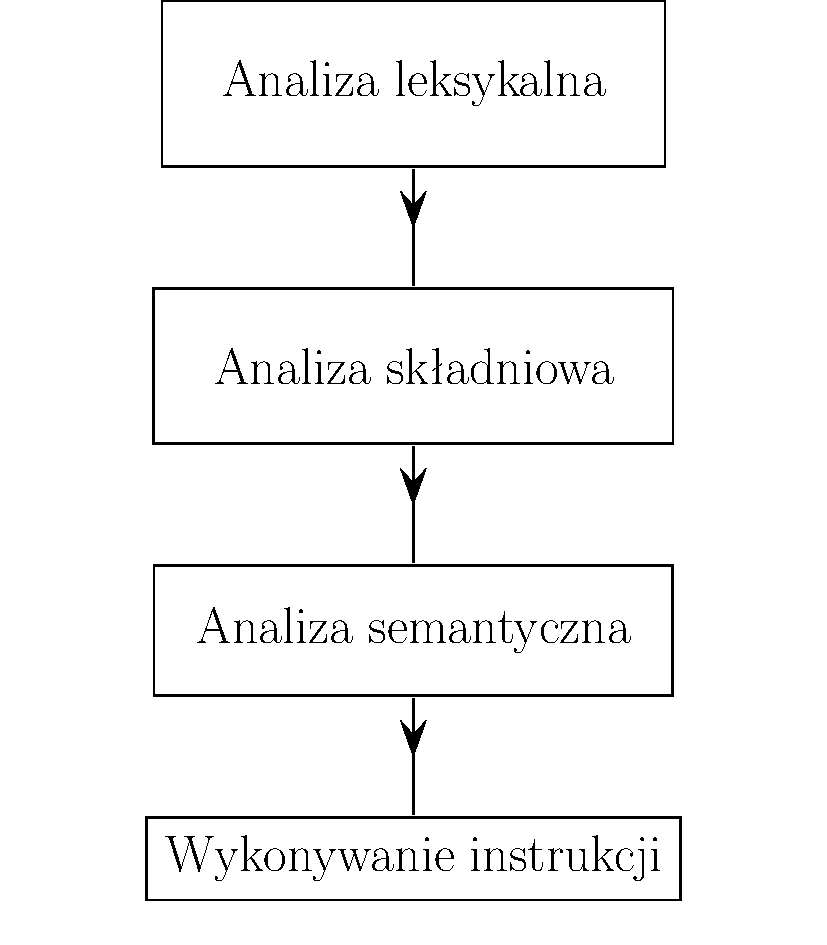
\includegraphics[width=0.7\textwidth, scale=0.5]{etapy.pdf}
  \end{center}
  \caption{Etapy tworzenie języka wysokiego poziomu. }
    \label{fig:etapy}
\end{figure}
\end{center}


\subsection{Analiza leksykalna} \label{p_leksykalna}

Zadaniem analizatora leksykalnego jest tworzenie symboli leksykalnych 
z przesłanego przez użytkownika strumienia znaków na wejście. 
Symbole te są następnie przesyłane  do analizatora składniowego. 
Symbole leksykalne tworzone są na podstawie tablicy wyrażeń regularnych i odpowiadającym i zadaniom,
czyli jeżeli przesłany strumień znaków należy do  n-tego wyrażenie regularne w tabeli 
 to zostanie wykonana powierzone mu zadanie, 
 którym na przykład
 może być \cite{aho}:
\begin{itemize}
 \item Nie wykonanie żadnego działania (strumień znaków zostanie pominięty)
 \item przesłanie symbolu leksykalnego do analizatora
 \item przesłanie symbolu leksykalnego wraz z ciągiem znaków, które należą do wyrażeniami
 \item przesłanie symbolu leksykalnego wraz z modyfikowanym ciągiem znaków
\end{itemize}

Podczas analiz leksykalne możemy zaprojektować analizator leksykalny, 
aby mógł wykrywać następujące błędy:
      \begin{itemize}
	\item   znaki pojawiające się na wejściu nie stanowią żadnego symbolu leksykalnego
	\item   jeśli na wejściu pojawi się znak nie nieobsługiwany 
	\item   gdy istniej możliwość przewidzenia błędnych ciągów znaków odpowiadające jakiemuś symbolowi leksykalnemu.
		Np. operator mniejszy równy \textquotedblleft$>=$\textquotedblright, 
		często jest pisany niepoprawnie w następujący sposób \textquotedblleft$=<$\textquotedblright.
		
		
      \end{itemize}

\subsection{Analiza składniowa} \label{p_skladniowa}


Analizator składniowy otrzymuje od analizatora ciąg symboli leksykalnych,
 które traktowane są jak symbole terminalne w gramatyce. Zadaniem analizatora składniowego,
 jest grupowanie symboli leksykalnych i tworzenie drzewa składniowego zgodnie
 z regułami gramatyki. 
Wynikiem działania analizatora składniowego jest drzewo składniowe lub wyświetlenie komunikatów o błędach.

Drzewem składniowym \ang{parse tree} nazywamy hierarchiczną strukturą danych,
 w której węzły odpowiadają:
\begin{itemize}
  \item  
    symbolu leksykalnemu, czyli skończonemu  ciągowi symboli terminalnych,
  \item  
    symbolu nieterminalnemu.
\end{itemize}


Najpopularniejszymi metodami wykorzystywanymi w analizatorach składniowych
 dla gramatyk są to metody zstępujące i wstępujące.
W metodzie zstępującej drzewo jest tworzone od korzenia do liści,
 a wstępującej odwrotnie od liści do korzenia.
W obu metodach wejście jest przeglądane od lewej strony.

Analizator składniowy może wykryć błędy w przypadku,
 gdy strumień symboli leksykalnych nie jest akceptowany przez gramatykę języka.
Jeżeli zostanie wykryty błąd to analizator składniowy powinien próbować odzyskać kontrolę w celu wykrycia kolejnych błędów
 i~poinformować o nich użytkownika.
Poniżej zostały następujące strategie\cite{aho}:
\begin{description}
  \item[Tryb paniki] --- 
     Po natrafieniu na błąd,
      analizator usuwa symbole leksykalne z wejścia, 
      aż natrafi na symbol z ustalonego zbioru od których może rozpocząć się dalsze poszukiwanie błędów.
  \item[Poziom frazy] --- 
     Pozwala zmienić lub dodać symbole leksykalne,
      które umożliwią dalsze dopasowania,
  \item [Produkcja dla błędu] --- 
     Jeżeli wiemy, 
      gdzie pojawiają się najczęściej błędy,
      to możemy dopisać odpowiednią regułę produkcji w gramatyce.
\end{description}

\subsection{Analiza semantyczna} \label{p_semantyczna}
Kolejnym etapem z rysunku \ref{fig:etapy} na stronie \pageref{fig:etapy} jest analiza semantyczna,
 której zadaniem jest sprawdzenie, 
 czy każdy identyfikator jakiegoś działania nazywany operatorem ma odpowiednią ilość składników nazywane argumentami.
Zadaniem analizatora semantycznego jest również sprawdzenie, czy każdy argument ma odpowiedni typ danych.
Wejściem do analizy semantycznej jest poprawnie zbudowane drzewo składniowe według gramatyk. \cite{aho}

 Błędy semantyczne możemy sklasyfikować w następujący sposób \cite{link_semantic}:
\begin{description}
 \item[Błędy krytyczne] ---
    błędy uniemożliwiające dalszą analizę 
 \item[Błędy tworzące nieoczekiwany] --- 
    istnieją błędy, które nie zostaną przechwycone i zostanie zwrócony nie oczekiwany wynik. Bardzo,
    częstym przykładem tego typu jest program napisany w języku C, który czyta nie ze swojej pamięci,
 \item[Niepotrzebnie rozbudowane polecenia] --- są to polecenia, które zostały podane nadmiarowe dane.
\end{description}


\begin{comment} 
\end{comment}
\chapter{Program}

\section{Opis implementacji programu}



Analiza leksykalna została zrealizowana, 
  przy użyciu narzędzia \textit{Lex},
  który został stworzony przez M. E. Lesk and E. Schmidt \cite{link_lex}.
Oprogramowanie to w znaczący sposób ułatwia tworzenie pierwszego etapu analizy,
 który został przedstawiony na rysunku \ref{fig:etapy} na stronie \pageref{fig:etapy} 
 i dodatkowo opisany  w podrozdziale \ref{p_leksykalna}
Poniżej został przedstawiony listing skryptu lex'a,
 który w całości realizuje owe zadanie.

\lstinputlisting[ label=l:lex, language=, caption = {Analiza leksykalna przy użyciu LEX'a.}] {"./skrypt/leksykalna.l"}


Tworzone symbole leksykalne są przekazywane do kolejnego etapu,
 który nazywamy analiza składniową. 
Polega ona na przekształceniu symboli leksykalnych, przy użyciu gramatyki w drzewo składniowe.
Na listingu \ref{l:gramatyka} został przedstawiony opis utworzonej gramatyki  
 w rozszerzonej notacja Backusa-Naura   \ang{ EBNF, Extended Backus-Naur Form},
 w której:
\begin{itemize}
 \item symbolami terminalnymi są:
\begin{verbatim}
EXIT  SAVE_DIR TABLE_NAME BASE_NAME USER_NAME
MAKE NUMBER IDENTIFIER 
CREATE KEY FACT DIMENSION SITE_WEB SITE_WEB_ADDRESS PGLOADER
LEFTPARENTHESIS RIGHTPARENTHESIS  SEMICOLON COMMA  LEX_ERROR 
\end{verbatim}
 \item symbolami nieterminalnymi są nazwy pisane małymi literami z prefiksem y\_
\end{itemize}

\lstinputlisting[ label=l:gramatyka, language=, caption = {Gramatyka języka w notacji EBNF.}] {"./tresc/EBNF.y"}


Etap ten został zrealizowany przy użyciu programu YACC,
 utworzonego przez Stephen C. Johnson.
Programy LEX i YACC, współpracują ze sobą, dzięki czemu tworzenie drzewa składniowego,
 którego definicja został podana w rozdziale \ref{p_skladniowa}, 
 staje się znacznie prostsza.
Na początku listingu  \ref{l:yacc},
 po słowach kluczowych token zostały przedstawione symbole leksykalne,
a w dalszej części pełna gramatyka tworzonego języka.
\lstinputlisting[ label=l:yacc, language=, caption = {Gramatyka języka w składni języka YACC.}] {"./skrypt/skladniowa.y"}  


W niniejszym programie sprawdzenie poprawności budowania drzewa składniowego,
 zostało zrealizowane przy użyciu testów jednostkowych \textit{cppunit}, 
 które powstały z wykorzystaniem biblioteki \textit{log4cpp}.

Program nie sprawdza poprawności atrybutów,
 ponieważ zajmują się tym systemy zarządzające bazą danych. 
Jeśli atrybuty będą nie poprawne,
 system zwróci odpowiedni komunikat. 
Dzięki takiemu rozwiązaniu program utworzony na potrzeby niniejszej pracy
 staje się wolny od ograniczeń związanych z dostępnymi typami w dowolnej bazie danych.
Odpowiedzialność za poprawne wpisywanie typów danych, zostaje przeniesiona na programistę,
 ponieważ to on powinien wiedzieć jakiego typu danych się oczekuje 
 i czy oczekiwany typ danych jest obsługiwany przez dany system zarządzania bazą danych.

Ostatnim etapem jest wykorzystanie drzewa składniowego w określony sposób. W naszym programie węzłem może być:

 \begin{itemize}
  \item ciąg znaków,
  \item klasa Tabela,
  \item klasa Kolumna,
 \end{itemize}
które są umieszczane w klasie Wprowadzone lub od razu zostają wykonywane na nich działania.

Działanie programu polega na przyjmowaniu ciągu znaków zakończonych symbolem średnika (;), które będziemy nazywać poleceniem.
Przykładowe polecenia mogą wyglądać następująco:

\begin{itemize}
 \item exit; --- 
    wyjście z programu.
 \item save\_dir --- 
    nazwa katalogu do zapisu, w folderze w którym został uruchomiony program.
 \item user\_name login;  ---
    login użytkownika bazy danych wykorzystywany przez skrypt pgloadera.
 \item base\_name nazwa; ---
    nazwa bazy danych wykorzystywana przez skrypt pgloadera.
 \item pgloader nazwa --- 
    utworzenie skryptu pgloadera. Nazwa odpowiada nazwie tabeli w hurtowni danych bez prefiksu inf\_. Przed użyciem wygenerowanego skryptu musi być zdefiniowana tabela intf\_nazwa.
 \item site\_web adres\_strony nazwa\_pliku ---
    tworzy skrypt linux'owy o rozszerzeniu *.sh z prefiksem dane, który został przedstawiony na listingu \ref{l:skrypt}, na stronie \pageref{l:skrypt}.
 \item make; ---
   Na podstawie zgromadzonych tabel wymiarów i jednej tabeli faktów wygenerowane zostają pliki sql, odpowiedzialne za tworzenie tabeli i kolejnych procesów zasilania.
\end{itemize}

Powyższe polecenia przesyłane są do analizy leksykalnej i składniowej. 
Wynikiem tych działań jest dodanie odpowiednich wartości do klasy Wyprowadzone lub od razu wykonanie danego działania.

 
\section{Przykładowe działania programu.}  \label{p_r_przyklady}

\subsection{Abstrakcyjny przykład schematu gwiazdy}
Na listingu \ref{l:wy_gwiazda} został przedstawiony abstrakcyjny przykład,
 którego schemat widoczny jest na rysunku \ref{fig:gwiazda}.
Pierwsze trzy linie zostały wyjaśnione w poprzednim podrozdziale.
Następnie utworzone zostają cztery tabele wymiarów i jedna faktowa (kolejność tutaj nie ma znaczenia). 
Zapisywane są one w klasie Wprowazdzone.
W linii 30 na omawianym listingu zostało wykorzystane plecenie \textit{make;},
 które generuje następujące pliki:
 
  \begin{itemize}
   \item 
      pliki z prefiksem \textit{create\_} są to pliki tworzące tabele dla odpowiednich procesów.
      Dla każdej tabeli wymiarów są to pliki 
        \begin{itemize}
         \item  create\_intf\_nazwa\_wymiaru,
         \item  create\_stg\_nazwa\_wymiaru,
         \item  create\_nazwa\_wymiaru,
            w naszym przykładzie mamy 4 tabele, więc powinniśmy otrzymać 12 plików 
            odpowiedzialnych za utworzenie dwunastu tabel
        \end{itemize}
      Dla tabeli faktów dodatkowo utworzona zostaje  jedna tabela create\_promo\_nazwa\_faktu,
      związku z tym otrzymujemy 4 pliki,
      łącznie mając ich 16. Program poinformuje nas o utworzonych plikach,
      tak jak zostało to zaprezentowane na listingu.
   \item 
      pliki, które nie zaczynają się od \textit{create\_},
      są plikami, wykorzystywanymi do cyklicznego zasilania.
     Kolejność tworzenia plików nie jest tutaj przypadkowa.
     Powinny być one uruchamiane w takiej kolejności, w jakiej zostały utworzone.
     Jest ich łącznie 11, po dwa dla każdego wymiaru i trzy dla faktu.
  \end{itemize}


%\lstinputlisting[ label=l:we_gwiazda, caption = { Przykład  .}] {"./przyklady/we_gwiazda.txt"}
\lstinputlisting[ label=l:wy_gwiazda, caption = {Przykład działania programu -- Schemat gwiazdy}] {"./przyklady/wy_gwiazda.txt"}
\subsection{Realizacja przykładu opisanego w rozdziale \ref{r_procesy}  }

W niniejszym podrozdziale został zaprezentowana realizacja omówionego przykładu w podrozdziale \ref{p_r_analiza_procesu}.
Poprzednim podrozdziale zostało wspomniane, że kolejność tworzenia tabel nie ma znaczenia,
 jest to spowodowane tym, że po słowach kluczowych  \textit{dimension} i  \textit{key} 
 podczas tworzenia kolumny musi wystąpić nazwa wymiaru. 
Jeżeli wymiar o tej nazwie nie zostanie zdefiniowany wcześniej to zostanie wygenerowany omówiony przykład.

W tabeli faktowej w kolumnie data\_notowania pojawiło się słowo kluczowe języka: key.
W ten sposób sygnalizujemy,
 że dana wartość jest kluczem w tabeli faktów
 i nie chcemy tworzyć dla nie klucza sztucznego. 

%\lstinputlisting[ label=l:we_np, caption = { Temat .}] {"./przyklady/we_np.txt"}
\lstinputlisting[ label=l:wy_np, caption = {Przykład działania programu -- Notowania GPW bez tabeli wymiarów.}] {"./przyklady/wy_np.txt"}


Na listingu \ref{l:wy_np2} została przedstawiona pełna realizacja owego przykładu.
Została w nim dodana tabela wymiarów,
 polecenie tworzące skrypt do pobierania
 i skrypt pgloadera.
Niestety pobierane dane do tabeli wymiarów wymagają modyfikacji,
 aby mogły być one załadowane do bazy danych przy użyciu skryptu pgloadera.
 Modyfikacje obejmują: 
\begin{itemize}
 \item usunięcie trzech pierwszych linii,
 \item usunięcie ostatniej linii,
 \item rozdzielenie kolumn znakiem 
\end{itemize}


%\lstinputlisting[ label=l:we_np2, caption = { Temat .}] {"./przyklady/we_np2.txt"}
\lstinputlisting[ label=l:wy_np2, caption = {Przykład działania programu -- Notowania GPW.}] {"./przyklady/wy_np2.txt"}



  
\chapter*{Podsumowanie}
\addcontentsline{toc}{chapter}{Podsumowanie}
Najważniejszym celem niniejszej pracy było stworzenie języka wysokiego poziomu wspomagającego 
 tworzenie procesów zasilających hurtownie danych.
Język ten odpowiada za częściową automatyzację pracy programisty, najbardziej powtarzalnych i najmniej ciekawych 
czynności, a zatem także najbardziej podatnych na błędy.

Dzięki pracy nad projektem języka wysokiego poziomu udało się osiągnąć zamierzony efekt,
 którym było zminimalizowanie ilości napisanego kodu,
 a tym samym zwiększenie efektywności pracy programisty. 
Osiągnięty cel potwierdzają listingi przykładowych użyć programu,
 które zostały zamieszczone w podrozdziale \ref{p_r_przyklady}. 

Stworzony na potrzeby pracy program posiada następujące cechy:

\begin{itemize} 
\item skrypt odpowiedzialny za pobranie pliku z danymi zostaje utworzony przy użcyiu jednego polecenia,
\item skrypt pgloader'a odpowiedzialny za załadowanie danych do bazy wygenerowany zostaje również przy użyciu jednego polecenia,
\item raz utworzona tabela wymiarów lub tabela faktów jest wielokrotnie wykorzystywana do tworzenia procesów zasilających,
\item automatycznie tworzone przez program tabele przejściowe i tabele docelowe pozwalają uniknąć błędów, które pojawiają
      się często podczas pisania kodu SQL,
\item język, w którym został napisany program jest prosty i intuicyjny, co pozwala uniknąć błędów składniowych.
\item elastyczność działania wynikająca z niezależności względem wykorzystywanego systemu bazodanowego. 
\end{itemize}

Dzięki wielu godzinom poświęconym hurtowniom danych,
 zauważyłem jak niewiele w tej dziedzinie zostało poświęcone odpowiednim procesom
automatyzującym i przyspieszającym tworzenie hurtowni danych.
Dzięki zdobytemu podczas pisania tej pracy doświadczeniu spostrzegłem
 jak istotne jest to zagadnienie dla dziedziny jaką są hurtownie danych i jak procesy usprawniające tworzenie hurtowni mogą wpłynąć
 na efektywność pracy programistów.
Dlatego też za cel obrałem sobie stworzenie języka wysokiego poziomu, który by tą pracę usprawniał, 
a zarazem czynił ją łatwiejszą. Program, który został napisany na potrzeby tej pracy dyplomowej może być wykorzystywany 
jako język generujący hurtownie danych "w locie" albo może po prostu usprawniać pracę programisty zajmującego się hurtowniami danych.

Tworzenie hurtowni danych jest procesem bardzo złożonym, dlatego perspektywa dalszego rozwoju języka daje również szerokie możliwości,
które nie kończą się bynajmniej na funkcjonalnościach opisanych w powyższej pracy.
Dostrzegam wiele potencjalnych funkcjonalności, o które można by rozbudować ten język. Do tych funkcjonalności zaliczam:

\begin{enumerate}
  \item stworzenie skryptu, którego zadaniem byłoby uruchamianie w sposób cykliczny utworzonych procesów zasilających,
  \item dodawanie lub usuwanie nowych elementów w warstwach procesów zasilających,
  \item zapisywanie informacji o utworzonych procesach w bazie danych w sposób umożliwiający 
        stworzenie zapytania zwracającego poprawną kolejność uruchamianych procesów,
  \item poszerzenie składni języka, która mogła by posłużyć do zapisywania
        ważnych informacji dotyczących tabel, dzięki czemu będzie możliwe automatyczne tworzenie częściowej dokumentacji w języku \LaTeX,
  \item utworzone pliki można by przechowywać na dysku w uporządkowanej strukturze katalogów,
  \item uniwersalność języka sprawia, że może być on w przyszłości rozwijany niezależnie od wykorzystywanego systemu bazodanowego.
\end{enumerate}


\listoffigures
\addcontentsline{toc}{chapter}{Spis rysunków}

\renewcommand\lstlistlistingname{Listingi kodu}
\addcontentsline{toc}{chapter}{Spis listingów}
\lstlistoflistings

\begin{thebibliography}{99}\addcontentsline{toc}{chapter}{Literatura}


\bibitem{TodMan}
Chris Todman, \textit{Projektowanie Hurtowni Danych. Wspomaganie zarządzania relacjami z klientem}, Wydawnictwa HELION 2011.
\bibitem{Inmon}
W.H. Inmon, \textit{Building the Data Warehouse, Fourth Edition}, Wydawnictwo Wiley Publishing, Inc. 2005
\bibitem{Kimball}  
Kimball R., Ross M., \textit{ The Data Warehouse Toolkit: The Complete Guide to Dimensional Modeling}, Wydawnictwo John Wiley and Sons, Inc. 2004
\bibitem{Vincent_Rainardi}
 Rainardi V.,  \textit{Building a data warehouse with exmaples in SQL server}, Wydawnictwo  Springer-Verlag New York, Inc. 2008
\bibitem{aho}
  Alfred V. Aho, Ravi Sethi, Jeffrey D. Ullman: \textit{Kompilatory}, Wydawnictwa Naukowo-Techniczne, Warszawa 2002
\bibitem{link_hd}
   \url{http://edu.pjwstk.edu.pl/wyklady/hur/scb/}
\bibitem{cube}
   \url{http://etl-tools.info/pl/bi/hurtownia_danych_schemat-gwiazdy.htm}
\bibitem{link_semantic}
   \url{http://dbs.informatik.uni-halle.de/sqllint/semerr_techrep.pdf}
\bibitem{link_eng_chomsky}
   \url{http://en.wikipedia.org/wiki/Chomsky\_hierarchy}
\bibitem{link_pl_chomsky}
   \url{http://pl.wikipedia.org/wiki/Hierarchia\_Chomsky'ego}
\bibitem{link_gramatyka}
   \url{http://en.wikipedia.org/wiki/Formal_grammar}
\bibitem{link_lex}
  \url{http://dinosaur.compilertools.net/}


\end{thebibliography}

\end{document}
